% !TEX encoding = UTF-8 Unicode

%%%%%%%%%%%%%%%%%%%%%%%%%%%%%%%%%%%%%%%%%%%%%%%%%%%%%%%%%%%%%%%%%%%%%%%%%%%%%%%%%%%%%%%%%%%%%%%%%%%%%%% 
%
% This TEST FILE should be run with asmeconf.cls version 1.40 (current CTAN release) or a later version.
%
% The result validates as PDF 2.0/A-4F under verapdf (https://demo.verapdf.org/) and the Arlington model (Arlington PDF 2.0 profile, ver.1.27.96)
% 		when run with pdfTeX, Version 3.141592653-2.6-1.40.26 (TeX Live 2024)
%
% The current class file loads an optional patch to address tagging with the caption package, [captionpatch], as described here:
%		https://github.com/latex3/tagging-project/issues/720#issuecomment-2386568711
%
% The current tagging code still yields the warning noted here:
%		https://github.com/latex3/tagging-project/issues/787#issue-2818240128
%
% Figures loaded as png, since original pdf versions are not compliant.
%	 
% The class file does NOT currently load unicode-math with lualatex, so that line of validation is not possible.
%		This will change in a future release.
%
% Date: 11 February 2025
%
%%%%%%%%%%%%%%%%%%%%%%%%%%%%%%%%%%%%%%%%%%%%%%%%%%%%%%%%%%%%%%%%%%%%%%%%%%%%%%%%%%%%%%%%%%%%%%%%%%%%%%% 


\DocumentMetadata{%
	tagging=on,
	pdfstandard=a-4f,
	pdfversion=2.0,
	lang=en-US,
}


% The rest is the asmeconf-template.tex (as in CTAN) with most language options removed.

%%%%%%%%%%%%%%%%%%%%%%%%%%%%%%%%%%%%%%%%%%%%%%%%%%%%%%%%%%%%%%%%%%%%%%%%%%%%%%%%%%%%%%%%%%%%%%%%%%%%%%% 
%%
%%  This file is asmeconf-template.tex, a LaTeX template to format ASME Conference papers according to
%%  the requirements on ASME's conference web pages, and including hypertext support for the pdf.
%%
%%  This file is version 1.40 dated 2025/01/29  
%%  
%%  As of version 1.11, this template defaults to ASME's newer conference guidelines first posted July 2019.
%% 			Those guidelines changed the requested author block formatting to be inline. 
%%			This LaTeX template continues to support the traditional grid format as a package option, [grid].
%%			Nomenclature now follows the abstract. Abstract text is set in italics.
%%
%%  Author: John H. Lienhard V
%%          Department of Mechanical Engineering
%%          Massachusetts Institute of Technology
%%          Cambridge, MA 02139-4307 USA
%%
%%  Class options include:
%%
%%          * An option to use the traditional grid arrangement of author names [grid].  
%%			*	 With this option, line breaks (\\) may be inserted into the address as needed. 
%%			*	 Author names that include commas should be enclosed in braces, e.g., {Joseph L. Smith, Jr.}.  
%%			*	 Authors may be grouped above a single affiliation using braces, e.g., {Henry Tudor, Catherine Parr}.
%%
%%          * An option to balance the heights of columns on the last page [balance]. 
%%          *    This option is NOT compatible with the [lineno] option.
%%
%%          * An option to include line numbers [lineno]. You must *run twice* for proper placement of the line numbers. 
%%			*	 The lineno package does not number titles, footnotes, captions, or tables.
%%          *    This option will disable balancing column height on final page if that option has been invoked.
%%          *    The lineno package won't always number the lines preceding displayed math in a paragraph because
%%          *    paragraph has not ended.  See that package's documentation for macros to address this problem, or
%%          *    just leave a blank line above the displayed equation while you are editing and then remove the 
%%          *    blank line and [lineno] option when you move to your final version.
%%
%%			* An option not to use boldface font for caption text [unboldcaption]
%%
%%          * Options to: 	omit the ASME copyright footer [nofoot]; 
%%			*				use government employee copyright notice [govt];
%%			*				use government contractor copyright notice [contractor]
%%			*				use copyright notice for some gov't employees [somegovt]
%%
%%          * Many options for calligraphic, script, and fraktur fonts from the mathalfa package; the
%%          *    example shown here is: [mathalfa=cal=boondoxo] to use the Boondox font for \mathcal.
%%          *    Some other options for cal are: dutchcal, zapfc, cm (default), euler,...
%%          *    frak (fraktur), bb (blackboard bold), scr (script) may also be chosen this way.
%%			*	 For details, refer to mathalfa documentation (at CTAN: https://www.ctan.org/pkg/mathalpha).
%%
%%          * Math options from M. Sharpe's newtxmath package: upright integrals [upint]; 
%%          *    [varvw] for a v and w that are better distinguished from Greek nu; and also 
%%          *    [subscriptcorrection, smallerops, varg, frenchmath, varbb, cmbraces, slantedGreek,...] 
%%			* 	 See newtx documentation for descriptions (at CTAN: https://www.ctan.org/pkg/newtx, v1.6 or higher is best).
%%
%%          * Option to for slightly larger small capitals, [largesc], from newtxtext package.
%%
%%          * An option to allow hyphenation of the typewriter font [hyphenate], from inconsolata package.
%%          *    Hyphenation is normally suppressed for typewriter mode because it is often used for code.
%%			*	 To replace the default variable word spacing by monospacing, use the option [mono].
%%			*	 To get a zero without a slash, use [var0]
%%
%%          * Options (used by the babel package) to include passages in languages other than English (e.g., a translation 
%%			*    of the abstract). Languages are called as options, e.g. [french], [spanish], [greek], [russian], etc. 
%%			*    See Appendix B for details. 
%%			*    Language support is most extensive when running LuaLaTeX, which automatically loads fontspec, but
%%			*	 be aware that you may to install additional fonts on your system to use fontspec.
%%			 
%%			* Option to use LuaLaTeX **without** bothering about extra fonts, [nofontspec]
%%
%%			* Legacy options for PDF/A compliance under pdftex: [pdf-a] will produce PDF/A-3u compliance with sRGB OutputIntent.
%%			*	 [pdfapart= 1 or 2 or 3] and [pdfaconformance= b or u] can enable levels 1b, 2b, 2u, and 3b.
%%			*
%%			*    Since 2022, LaTeX has included integrated support for pdf-a, through the \DocumentMetadata{..}
%%			*    command.  This preferred approach works with both pdfTeX and luaLaTeX. The asmeconf class supports this feature, 
%%			*	 which obviates the aforementioned class options. (An up-to-date LaTeX installation is required.)
%%
%%  The use of commands defined or modified by the asmeconf class is illustrated throughout this file. In particular, 
%%  ASME requires capitalized, sans-serif section headings, and as a result some care is needed when using macros 
%%  in section headings, as also illustrated below.
%%
%%  Use an up-to-date and complete installation of LaTeX, such as TeX Live 2020 or later. Errors may occur with old set-ups.
%%
 %=========================================================
%% 
%% LICENSE: 
%%
%% Copyright (c) 2025 John H. Lienhard
%%
%% Offered under the MIT license: https://ctan.org/license/mit 
%%
%%%%%%%%%%%%%%%%%%%%%%%%%%%%%%%%%%%%%%%%%%%%%%%%%%%%%%%%%%%%%%%%%%%%%%%%%%%%%%%%%%%%%%%%%%%%%%%%%%%%%%% 

%%%%%%%%%%%%%%%%%%%%%%%%%%%%%%%%%%%%%%%%%%%%%%%%%%%%%%%%%%%%%%%%%%%%%%%%%%%%%%%%%%%%%%%%%%%%%%%%%%%%%%%

%% Class options are described above. Change these options as desired. 
%%		If you are not using the language options, remove them (together with Appendices B and C)
%%	 	Remove the [colorlinks] option before *final* submission to ASME, to get black text for printing,
%%		but keep that option for other uses.
 
\documentclass[captionpatch,colorlinks,upint,subscriptcorrection,varvw,mathalfa=cal=boondoxo,german]{asmeconf}

%%%%%  pdf metadata  %%%%%%%%%%%%%%%%%%%%%%%%%%%%%%%%%%%%%%%%%%%%%%%%%%%%%%%%%%%%%%%%%%%%%%%%%%%%%%%%%%

\hypersetup{%
	pdfauthor={John H. Lienhard},									  % <=== change to YOUR name
	pdftitle={ASME Conference Paper LaTeX Template},                  % <=== change to YOUR pdf file title
	pdfkeywords={ASME conference paper, LaTeX template, BibTeX style},% <=== change to YOUR pdf keywords
	pdfsubject = {Describes the asmeconf LaTeX template},			  % <=== change to YOUR subject
%	pdfurl={https://ctan.org/pkg/asmeconf},% may delete
	pdflicenseurl={https://ctan.org/pkg/asmeconf},% may delete
}


%%%%%%%%%%%%%%%%%%%%%%%%%%%%%%%%%%%%%%%%%%%%%%%%%%%%%%%%%%%%%%%%%%%%%%%%%%%%%%%%%%%%%%%%%%%%%%%%%%%%%%%

\begin{document}

% Change these fields to the right content for your conference.
% You can comment these out if for some reason you don't want a header.
% Use title case (first letters capitalized), not all capitals

\ConfName{Proceedings of the ASME 2025\linebreak International Mechanical Engineering Congress and Exposition}
\ConfAcronym{IMECE2025}
\ConfDate{November 16--20, 2025} % update 
\ConfCity{Memphis, TN} % update 
\PaperNo{IMECE2025-XXXX}

% Units of measure (e.g., cm) and other specialty lowercase terms in the title should be 
%   enclosed in \NoCaseChange{...} to maintain lower case type
%   LaTeX will automatically set the rest of the title in all capital letters.

\title{A LATEX Template for ASME Conference Papers: \NoCaseChange{\texttt{asmeconf.cls}}} % <=== replace with YOUR title
%\title{Place Title Here: Place Subtitle After Colon} 
 
%   Put author names into the order you want. Use the same order for affiliations.
%   \affil{#} tags the author's affiliation to the address in \SetAffiliation{#}.
%   No space between last name and \affil{#}, separate names with commas.
%
%	For a sole author or a single affiliation for all authors, {#} may be left empty, as \affil{} and \SetAffiliation{} (but not with [grid] option!)
%
%   \CorrespondingAuthor{email} follows that author's affiliation, no spaces before or after 
%   If multiple corresponding authors, put both email addresses in the same command and place after both authors.
%
%   \JointFirstAuthor, if applicable, follows the affiliation of the relevant authors, no spaces.

\SetAuthors{%
    John H. Lienhard\affil{1}\JointFirstAuthor\CorrespondingAuthor{}, 
	Luis Hern\'andez\affil{2}\JointFirstAuthor, 
	Maria Silva\affil{3}, 
	Henry Tudor\affil{4},  
	Catherine~Parr\affil{4}\CorrespondingAuthor{lienhard@mit.edu, kate@thepalace.gov}
	}

\SetAffiliation{1}{Massachusetts Institute of Technology, Cambridge, MA}
\SetAffiliation{2}{Institution or Company Name, City, State}
\SetAffiliation{3}{Institution or Company Name, City, Province, Canada}
\SetAffiliation{4}{Hampton Court Palace, Richmond, England}
%	Note: Luis and Maria are not real people.  Henry and Catherine have been dead for >450 years.
%   Note: You can force a line break in the address using \\ 

%	To switch from inline author names to gridded names, use the [grid] option.

\maketitle

%%% Use this footnote for tracking various versions of your draft. Change text to suit your own needs. 
%%% \date{..} calls the same command. 
\versionfootnote{Documentation for \texttt{asmeconf.cls}: Version~\versionno, \today.}% <=== Delete before final submission.

%%% Change these to your keywords.  Keywords are automatically printed at the end of the abstract.
%%% This command MUST COME BEFORE the end of the abstract.
%%% If you don't want keywords, leave the argument of \keywords{} empty (or use the abstract* environment)

\keywords{ASME conference paper, \LaTeX\ Template, \hologo{BibTeX}}

%%%%%  End of fields to be completed. Now write your paper. %%%%%%%%%%%%%%%%%%%%%%%%%%%%%%%%%%%%%%%%%%%

%%%%%  ABSTRACT  %%%%%%%%%%%%%%%%%%%%%%%%%%%%%%%%%%%%%%%%%%%%%%%%%%%
%%
%% Abstract should be 200 words or less
\begin{abstract}

This paper is an example of and a  {\upshape\LaTeX} template for typesetting ASME conference papers using the {\upshape\texttt{asmeconf}} class. This  {\upshape\LaTeX} template follows ASME guidelines for margins, fonts, headings, captions, and reference formats as of 2025. The class is intended to be used with the {\upshape\texttt{asmeconf.bst} \hologo{BibTeX}} style for reference formatting, which is part of this distribution. The template produces pdfs that contain hyperlinks, bookmarks, and metadata; and references can include the DOI and URL fields. Links may be colored, for online use, or black, for publication. The class enables inline author names, following ASME's current style, but can also produce the traditional grid style. Options include line numbering, final column balancing, various math options, government copyright, and archivability (PDF/A). In addition, section headers may contain mathematics, references, citations, and footnotes. The class is compatible with {\upshape\hologo{pdfLaTeX}} or {\upshape\hologo{LuaLaTeX}}.
\end{abstract}

%%%%%%%%%  NOMENCLATURE (OPTIONAL) %%%%%%%%%%%%%%%%%%%%%%%%%%%%%%%%%
%%
%% To change space between the symbols and  definitions, use \begin{nomenclature}[Xcm] where X is a number 
%% The unit cm can be replaced by any LaTeX unit of dimension: pt, in, ex, em, pc, etc.
%% Default is 2em.
%% \EntryHeading{..} produces an italicized subheading in the nomenclature list, e.g., \EntryHeading{Greek letters}

\begin{nomenclature}
\EntryHeading{Roman letters}
\entry{$k$}{Thermal conductivity [W m$^{-1}$ K$^{-1}$]}
\entry{$\vec{q}$}{Heat flux vector [W m$^{-2}$]}

\EntryHeading{Greek letters}
\entry{$\alpha$}{Thermal diffusivity [m$^2$ s$^{-1}$]}
\entry{$\nu$}{Kinematic viscosity [m$^2$ s$^{-1}$]}

\EntryHeading{Dimensionless groups}
\entry{Pr}{Prandtl number, $\nu/\alpha$}
\entry{Sc}{Schmidt number, $\nu/\mathcal{D}_{1,2}$}

\EntryHeading{Superscripts and subscripts}
\entry{b}{bulk value}
\entry{$\infty$}{free stream value}
\end{nomenclature}

%%%%%%%%%  BODY OF PAPER %%%%%%%%%%%%%%%%%%%%%%%%%%%%%%%%%

\section{Introduction}
The \texttt{\hrefurl{https://ctan.org/pkg/asmeconf}{asmeconf}} class typesets papers with margins, fonts, headings, captions, and reference formats that follow the specifications for conference papers of the American Society of Mechanical Engineers (ASME). In contrast to older ASME \LaTeX\ templates, \texttt{asmeconf} will set internal and external hyperlinks, and the pdf file will contain bookmarks and metadata. Many other useful features have been incorporated. This class is not a publication of ASME, but the author has published in ASME conferences since 1983. 

The \texttt{.tex} file may be written using standard \LaTeX\ commands, although some specific initial commands are needed to format the blocks containing the author[s], title, and abstract.  This class loads a number of other packages, all of which are contained in up-to-date versions of \hrefurl{https://www.tug.org/texlive/}{\TeX\ Live}, \hrefurl{http://www.tug.org/mactex/}{Mac\TeX}, and similar platforms. If you get an error message about a missing package, you may download it at no cost from CTAN (\hrefurl{https://ctan.org}{ctan.org}). 

\subsection{Essential Initial Commands}

To begin, fill in the fields to be completed at top of the \texttt{asmeconf-template.tex} file. These fields include the headers for your conference and your paper number. Specified metadata will be placed into the pdf file itself. 
The title should be placed into \verb|\title{..}|. 

Put author names into the \verb|\SetAuthors{name, name,...}| command in the desired order; follow the syntax illustrated \texttt{asmeconf-template.tex} file. Put each distinct address sequentially into a separate \verb|\SetAffiliation{n}{address}|, where $n = 1,2,\ldots$ Tag each author with an affiliation by putting \verb|\affil{n}| after that author's name inside the \verb|\SetAuthors{..| command. 

Keep author addresses short.  List the author institution, and the City, State (US authors), City, Province, Canada (Canadian authors), or City, Country (other international authors). 

One author (or more) may be designated as the corresponding author by placing \verb|\CorrespondingAuthor{email}|  after \verb|\affil{n}|. Two or more authors may be joint first authors by putting \verb|\JointFirstAuthor| after \verb|\affil{n}|.

After setting up the headers, authors,  and title, issue the \verb|\maketitle| command. 

The abstract text must be placed into \verb|\begin{abstract}| \ldots \verb|\end{abstract}|. The abstract will automatically be italicized. Keywords may be included using the \verb|\keywords{..}| command. The \texttt{keyword} command \textit{must} be issued before the abstract environment. 

%%%%%%%%%%%%%%%%%%%%%%%%%%%%%%%%%%%%%%%%%%%%%%%%%%%%%%%%%%%

\section{Referring to Citations, Figures, and Equations}

Citations are automatically numbered \cite{ning2002}. They should be inserted in the text using a \verb|\cite{ref}| command~\cite{gibson2008,stevens1999}. The citations will be automatically sorted and compressed if they are given in a set \cite{stevens1999,ning2002,gibson2008,wions2005,smith2002,watson1982}. 
A specific reference may be named with an abbreviation, as in Ref.~\cite{watson1982}.
See the \texttt{asmeconf-sample.bib} file and Sect.~\ref{sec:references} for examples of entering references.

For ASME conference papers, the labels Equation and Figure should be abbreviated when they do not start a sentence, as in  Eq.~\eqref{eqn:dw} and Fig.~\ref{fig:1}. Figure~\ref{fig:1} is spelled out when it starts a sentence. Equation~\eqref{eqn:dw} is spelled out when it starts a sentence. 

Equations are typeset in the usual way and will be automatically numbered.  The class file loads the \texttt{amsmath} and \texttt{mathtools} packages. Further, the \texttt{newtxmath} package used for the math fonts includes many additional features (see Sect.~\ref{sec:moremath}).
\begin{equation}\label{eqn:fourier}
\vec{q} = -k\nabla T
\end{equation}

ASME prefers SI units. (U.S.\ style units may follow in parentheses.) Be sure to put all symbols into the nomenclature list, including their units.


%%%%%%%%%%%%% begin figure %%%%%%%%%%%%%%%%%

%% captions go below figures

\begin{figure}
\centering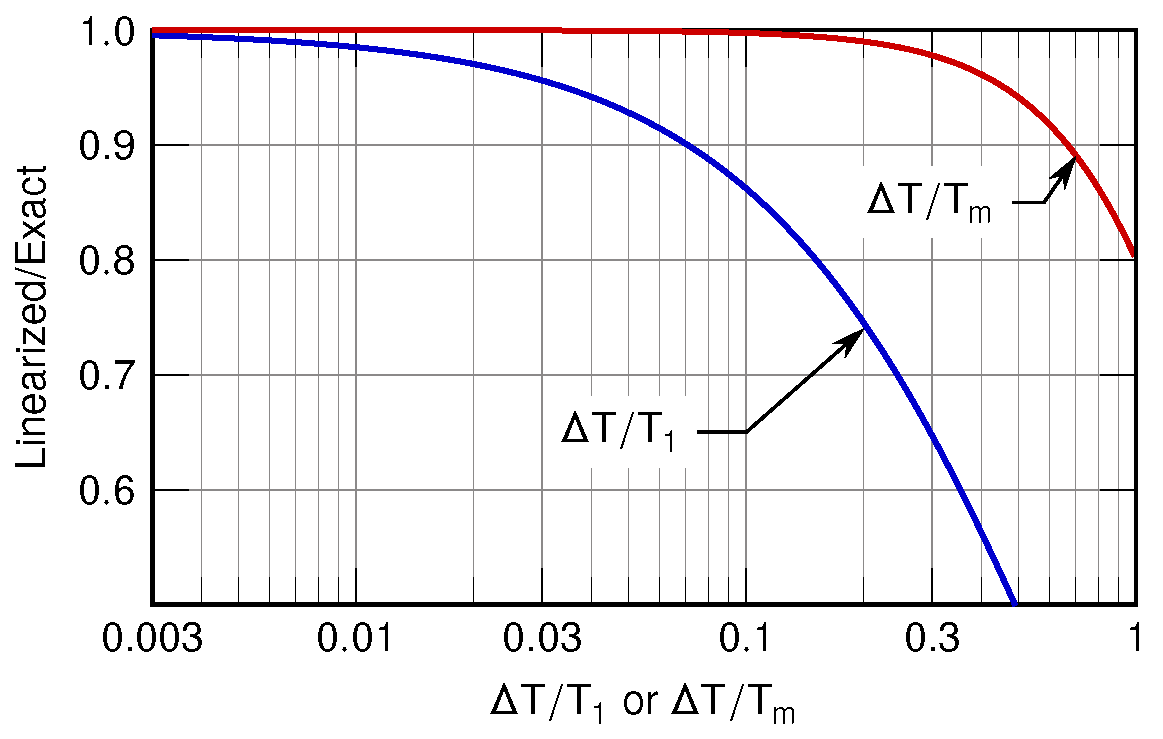
\includegraphics[width=\linewidth, alt = {Linearization error in radiant flux}]{sample-figure-1.png}
\caption{Caption with math, eqn.~\eqref{eqn:fourier}: $\Delta T/T_m$ vs.\ $\Delta T/T_1$~\cite{Lienhard2019}}\label{fig:1}
\end{figure}
 
%%%%%%%%%%%%% end figure %%%%%%%%%%%%%%%%%%%


%%%%%%%%%%%%%%%%%%%%%%%%%%%%%%%%%%%%%%%%%%%%%%%%%%%%%%%%%%%

%% Use title case for subsections and subsubsections (first letter of words capitalized)

\section{Section Headings and Captions}

ASME requires that section headings and captions be set in an uppercase, sans serif font.  The class will do this automatically.  You can place \verb|\cite{..}|, \verb|\ref{..}|, \verb|\label{..}|, and mathematics into headings and captions directly, as you would in the main text. Do not enclose them braces, e.g.\ \verb|{\cite{..}}|, which will cause errors. You can place \verb|\footnote{..}| into headings, but not into captions.\footnote{See \texttt{tex-stackexchange} for various approaches to footnotes in captions, if they seem necessary. For footnotes in tables, use the \texttt{tablefootnote} package.}\footnote{Sequential footnotes are automatically separated by a comma.}

Text in section headings and captions will not be capitalized if enclosed in a \verb|\NoCaseChange{..}| command.

Sections may either be numbered or left unnumbered.

Simple mathematical expressions can be used in either captions or section headings. For a section heading that includes more complicated math (and macros), you may use the optional argument of \verb|\section[..]{..}| to create a pdf bookmark without losing characters or producing warnings or errors. See the \texttt{asmeconf-template.tex} source file for examples of this procedure. These bookmarks should usually be text expressions, although some math is supported.  

To eliminate boldface type in caption text and math, use the class option \texttt{[unboldcaption]}.  To avoid \texttt{sans} math in captions, put \verb|\NoCaseChange{\mathversion{normal}}| in the caption.

\subsection{Subsection and Sub-subsection Headings}

Subsections and sub-subsection headings should be entered in title case, with the first letter of primary words capitalized. Sub-subsections (i.e., paragraphs) are never numbered.


%%%%%%%%%%%%%%% begin simple table %%%%%%%%%%%%%%%%%%%%%%%%%% 

%% Captions go above tables
%%
%% Note that placement of figures and tables can managed with the [!tbhp] options. See: https://latexref.xyz/dev/latex2e.html#Floats

\begin{table}[t]
\caption[Table]{A simple table}\label{tab:1}
\centering{%
\begin{tabular}{llr}
\toprule
Experiment & $u$ [m/s] & $T$ [\textdegree C] \\
\midrule
Run 11 & 12.5 & 103.4 \\
Run 12 & 24   & 68.3 \\
\bottomrule
\end{tabular}
}
\end{table}

%%%%%%%%%%%%%%%% end table  %%%%%%%%%%%%%%%%%%%%%%%%%%%%%%%%%%%% 

%%%%%%%%%%%%%%% begin more complicated table %%%%%%%%%%%%%%%%%%%%%%%%%%%%%%%%%%%%

% note column set as a 3 cm wide paragraph with 1em hanging indentation. See array package documentation.
% note numbers centered on "." (with d{3.3}) and on "," (with ,{3.3}).  See dcolumn package documentation.
\begin{table}[t]
\caption{Table with more complicated columns}\label{tab:2}%
\centering{%
\begin{tabular}{!{\hspace*{0.5cm}} >{\raggedright\hangindent=1em} p{3cm} d{3.3} @{\hspace*{1cm}} ,{3.3} !{\hspace*{0.5cm}}}
\toprule
Experiment & \multicolumn{1}{c@{\hspace*{1cm}}}{$u$ [m/s]} & \multicolumn{1}{c!{\hspace*{0.5cm}}}{$T$ [\textdegree C]} \\
\midrule
The first test we ran this morning   & 124.3     &   68,3   \\
The second test we ran this morning  &  82.50    &  103,46  \\
Our competitor's test                &  72.321   &  141,384 \\
\bottomrule
\end{tabular}
}
\end{table}

%%%%%%%%%%%%%%%% end table  %%%%%%%%%%%%%%%%%%%%%%%%%%%%%%%%%%%% 

%%%%%%%%%%%%%%% begin two column table %%%%%%%%%%%%%%%%%% 
\begin{table*}
\caption{A table spanning two columns}\label{tab:3}%
\centering{%
\begin{tabular*}{0.8\textwidth}{@{\hspace*{1.5em}}@{\extracolsep{\fill}}ccc!{\hspace*{3.em}}ccc@{\hspace*{1.5em}}}
\toprule
\multicolumn{1}{@{\hspace*{1.5em}}c}{$x$\rule{0pt}{11pt}} &
\multicolumn{1}{c}{$\textrm{erf}(x)$} &
\multicolumn{1}{c!{\hspace*{3.em}}}{$\textrm{erfc}(x)$} &
\multicolumn{1}{c}{$x$} &
\multicolumn{1}{c}{$\textrm{erf}(x)$} &
\multicolumn{1}{c@{\hspace*{1.5em}}}{$\textrm{erfc}(x)$} \\ \midrule
0.00 & 0.00000 & 1.00000 & 1.10 & 0.88021 & 0.11980\rule{0pt}{11pt} \\
0.05 & 0.05637 & 0.94363 & 1.20 & 0.91031 & 0.08969 \\
0.10 & 0.11246 & 0.88754 & 1.30 & 0.93401 & 0.06599 \\
0.15 & 0.16800 & 0.83200 & 1.40 & 0.95229 & 0.04771 \\
0.20 & 0.22270 & 0.77730 & 1.50 & 0.96611 & 0.03389 \\
0.30 & 0.32863 & 0.67137 & 1.60 & 0.97635 & 0.02365 \\
0.40 & 0.42839 & 0.57161 & 1.70 & 0.98379 & 0.01621 \\
0.50 & 0.52050 & 0.47950 & 1.80 & 0.98909 & 0.01091 \\
0.60 & 0.60386 & 0.39614 & 1.82\makebox[0pt][l]{14} & 0.99000 & 0.01000 \\
0.70 & 0.67780 & 0.32220 & 1.90 & 0.99279 & 0.00721 \\
0.80 & 0.74210 & 0.25790 & 2.00 & 0.99532 & 0.00468 \\
0.90 & 0.79691 & 0.20309 & 2.50 & 0.99959 & 0.00041 \\
1.00 & 0.84270 & 0.15730 & 3.00 & 0.99998 & 0.00002 \\[2pt]
\bottomrule\end{tabular*}
}
\end{table*}

%%%%%%%%%%%%%%%%% end two column table  %%%%%%%%%%%%%%%%%%%%%%%%%%%%%%% 

%%%%%%%%%%%%%%%%%%%%%%%%%%%%%%%%%%%%%%%
\section{Tables and Figures}

Table \ref{tab:1} is an example of a simple table. Table captions should be placed above tables.
The class loads the \texttt{booktabs} package (used for horizontal rules in Tables \ref{tab:1} and \ref{tab:2}), and the \texttt{array} and \texttt{dcolumn} packages which provide extended capabilities for columns in the \texttt{tabular} environment (see Table \ref{tab:2}).  Table \ref{tab:3} is an example of a table that spans two columns. Two column tables (and figures) will always float to the top of a later page.

Figure captions go below figures. Figure~\ref{fig:2} is an example of a figure that spans two columns and includes subfigures. The text in figures (and tables) should be no smaller than 6~point type. Images in figures are handled by the standard \texttt{graphicx} package.

Landscape figures and tables may be produced at full-page size by putting \verb|\usepackage[figuresright]{rotating}| in your \texttt{.tex} file's preamble and using the \texttt{sidewaystable*} and \texttt{sidewaysfigure*} environments~\cite{fairbairns}.


%%%%%%%%%%%%%%%%%%%%%%%%%%%%%%%%%%%%%%%%%%%%%%%%%%%%%%%%%%%%%%%%%%%%%%

\section{Reference Formatting with \NoCaseChange{\texttt{asmeconf.bst}}\footnote{To prevent capitalization of text in a section heading or caption, such as an SI unit, enclose it in a \texttt{\textbackslash NoCaseChange} command. As of the July 2022 release of \LaTeX, commands used in a heading or caption may be protected globally by putting this in the preamble: \texttt{\textbackslash AddToNoCaseChangeList\{\textbackslash MyCommand\}}.}}\label{sec:references}

The {\upshape\texttt{asmeconf.bst}} \hologo{BibTeX}  style follows the reference styles shown on ASME's conference web site in  2022.\footnote{\texttt{asmeconf.bst} is intended as a replacement for the old \texttt{asmems4.bst}, which does not follow ASME's current reference formats or support DOI and URL.}
Examples for these and many other cases are given in the \texttt{asmeconf-sample.bib} file, which is part of this distribution. Citations and references are managed by the standard \texttt{natbib} package.  Nevertheless, a few comments are necessary. 

%% sub-subsections should *not* be numbered according to ASME's style

\subsubsection*{DOI, URL, and eprint} Include DOI numbers when they are available.  URL's may alternatively be given. ASME requests that URLs point to a document's abstract.

Basic support for \texttt{eprint} numbers is also included, generating a url at the end of the citation. The \texttt{archive} type may be specified using the macros \texttt{arxiv, google\-books, hdl, jstore, oclc}, or \texttt{pubmed} (e.g., \texttt{archive=hdl},  \textit{without} braces). Both \texttt{eprint} and \texttt{archive} fields \textit{must} be given. Other root urls may be invoked using \verb|archive = {https://another.url.org/}|.

\subsubsection*{Online Sources} A bibliography entry \verb|@online{..| is included for citation of online sources, such as web pages. A \texttt{url} or \texttt{eprint} with \texttt{archive} must be included. See the examples of use in the \texttt{asmeconf-sample.bib} file. 

\subsubsection*{Date Accessed} The \verb|urldate={..}| field may be used to provide the date on which a given url was accessed. By default, the text printed will be \texttt{Accessed `date',}. The word ``Accessed'' may be changed using the \verb|urltype={..}| field.

\subsubsection*{Conference Location and Date.} To specify the city and date of a conference, you can use \verb|venue={..}| and \verb|eventdate={..}| with the entries \verb|@inproceeedings{..| and \verb|@proceeedings{..|.

\subsubsection*{Capitalization of Titles} ASME's bibliography style requires that document titles be in title case. The first letters of principal words are capitalized. Do this in the \texttt{.bib} file.



%%%%%%%%%%%%%%%%%  begin two column figure  %%%%%%%%%%%%%%%%%%%%%%%%%%%

\begin{figure*}
\begin{subfigure}[b]{\columnwidth}% subfigure is basically the same as minipage
\centering{
  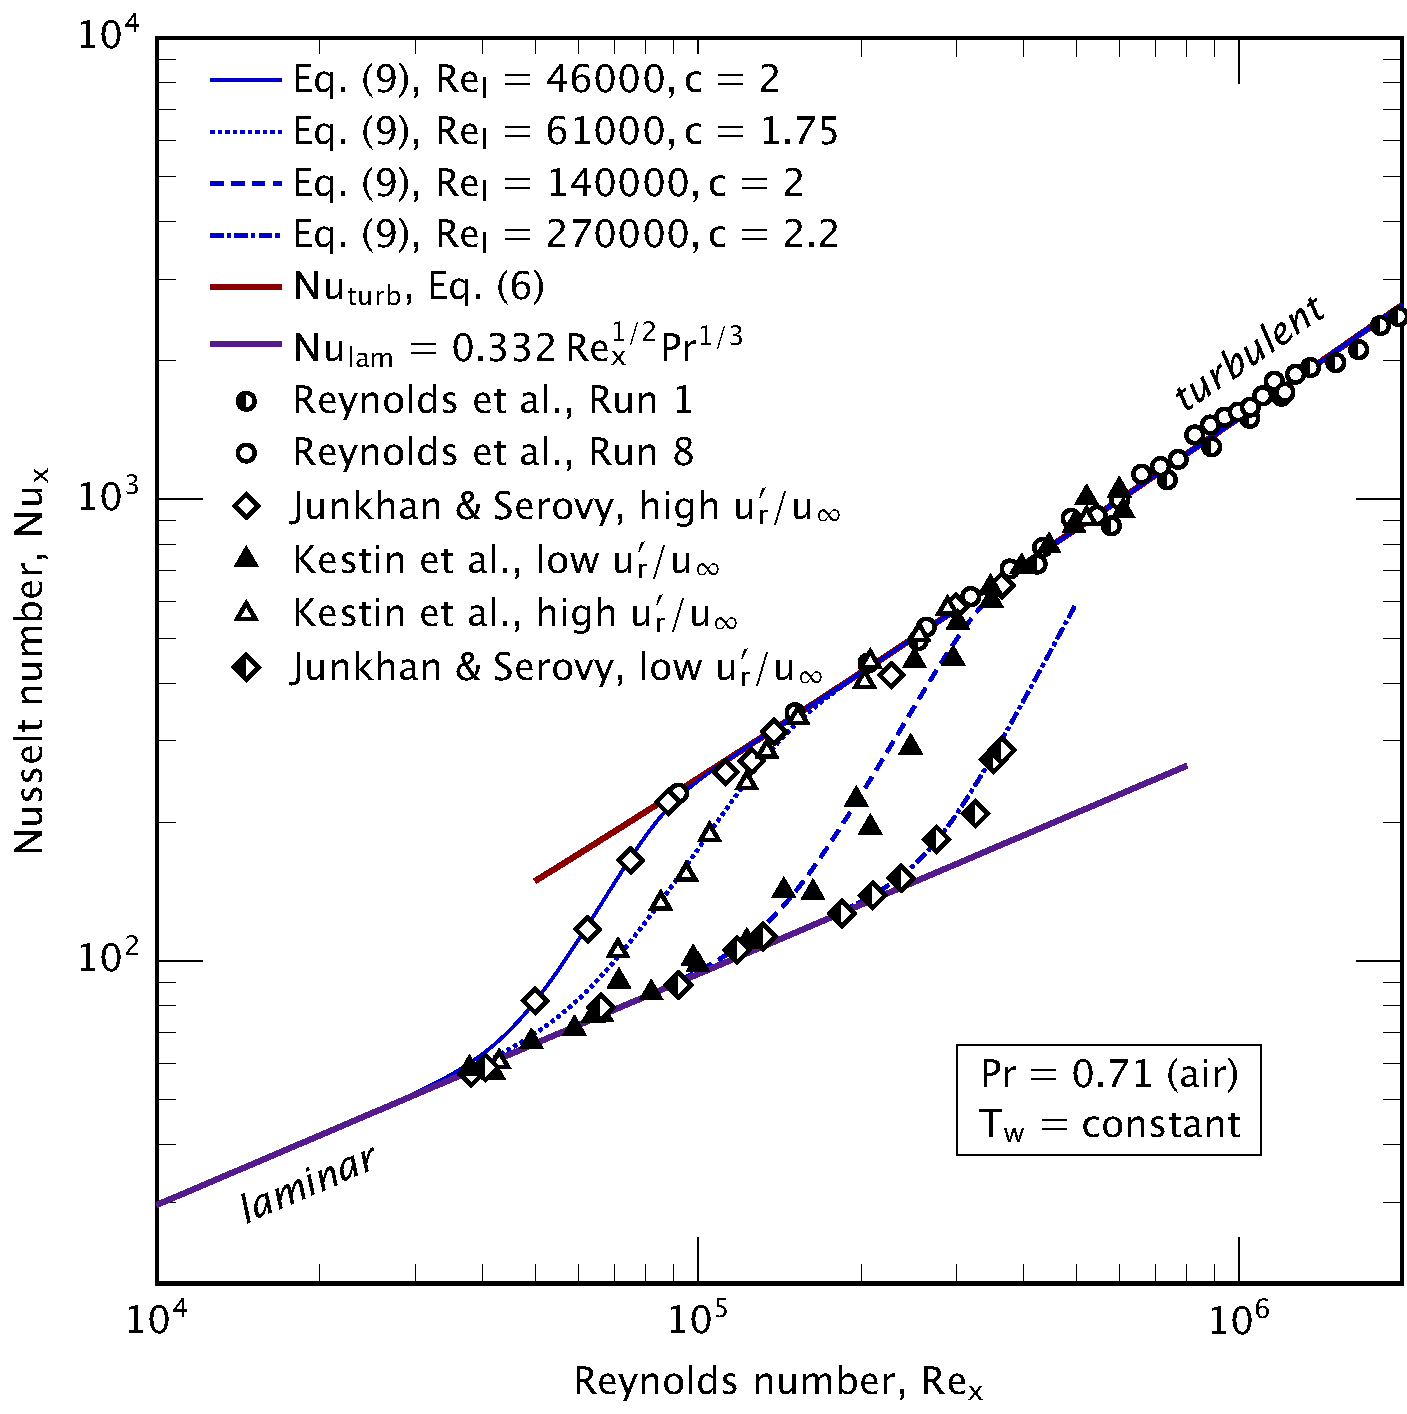
\includegraphics[width=0.9\linewidth, alt={Nusselt number data for isothermal wall}]{sample-figure-2a.png}%
}
\subcaption{Uniform temperature wall\label{fig:isothermal}}
\end{subfigure}%
\hspace*{\columnsep}% with this space added, puts each figure at column center
%%%%%%%%%%%%% no line break between these two subfigures
\begin{subfigure}[b]{\columnwidth}
\centering{%
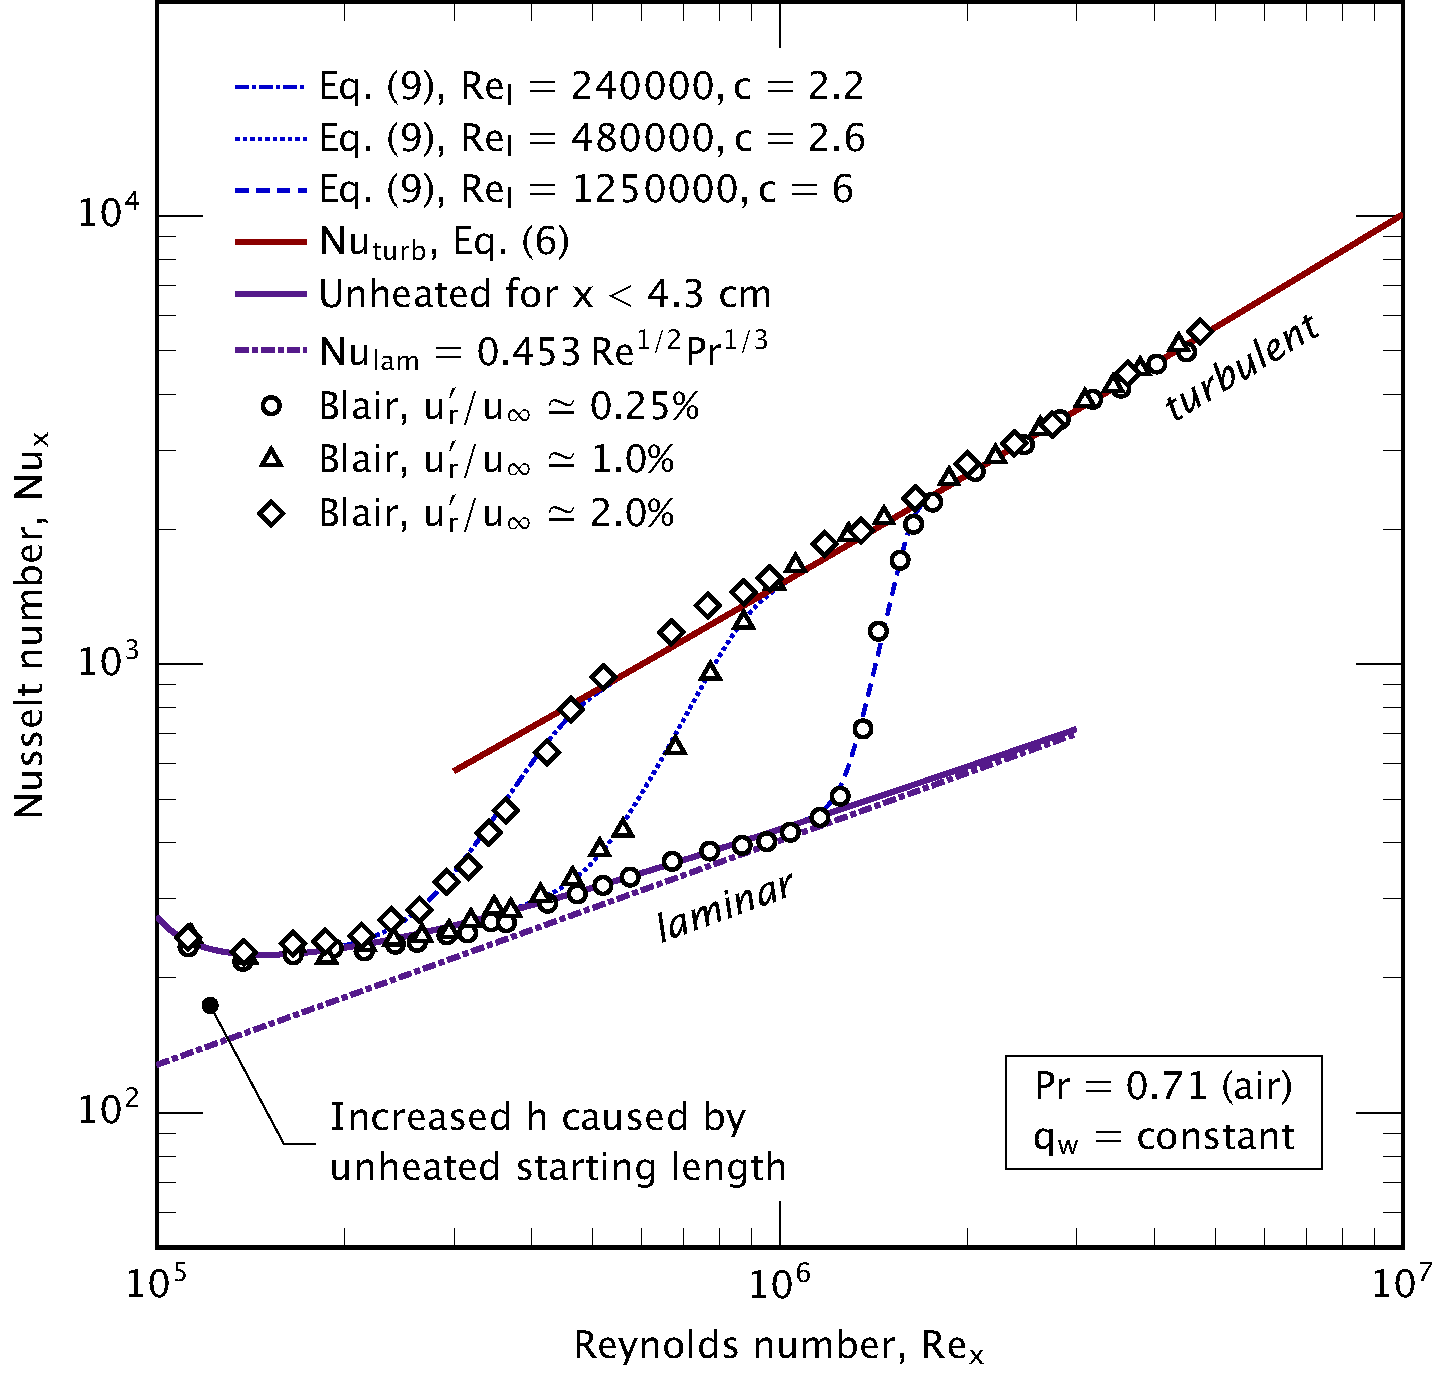
\includegraphics[width=0.927\linewidth, alt={Nusselt number data for uniform heat flux wall}]{sample-figure-2b.png}%
}%
\subcaption{Uniform heat flux wall with unheated starting length\label{fig:uniform-flux}}
\end{subfigure}
\caption{A figure with two subfigures~\cite{lienhard2020}\label{fig:2}}
\end{figure*}

%%%%%%%%%%%%%%%%%%%  end two column figure  %%%%%%%%%%%%%%%%%%%%%%%%%%


%%%%%%%%%%%%%%%  MORE ON MATH   %%%%%%%%%%%%%%%%%%%%%%%%%%%%%%%%%%%%%%%%%%%%%%%%%%%%%%%%%%%%%%%%%%%%%%

%% Here is an example of managing complicated math in a section or subsection heading: 
%%    the optional argument to \section will provide the pdf bookmark
%%    without losing characters or producing warnings/errors.
%%
%% In this heading, letter u is forced to be upright with \mathrm{u}
%%
\section[More on math: u\cdot\omega=0]{More on math: $\vec{\mathrm{u}}\cdot\vec{\omega}=0$}\label{sec:moremath}

In most cases, the need for a wide equation can be eliminated by using one of the multiline equation environments defined by 
\texttt{amsmath}, such as \texttt{align}, \texttt{split}, or \texttt{multline}~\cite{amsmath}. The following equation is set with the 
\texttt{multline} environment:
\begin{multline}\label{eqn:energy}
\frac{\partial}{\partial t}\left[\rho\bigl(e + \lvert\vec{u}\rvert^2\big/2\bigr)\right]  + \nabla\cdot\left[\rho\bigl(h + \lvert\vec{u}\rvert^2\big/2 \bigr)\vec{u}\right] \\
 ={}-\nabla \cdot \vec{q} +  \rho \vec{u}\cdot\vec{g}+ \frac{\partial}{\partial x_j}\bigl(d_{ji}u_i\bigr) + \dot{Q}_v
\end{multline}
An example using \texttt{align} appears in Appendix~\ref{appendix:a}.

An alternative solution may be to set large equations into two-column-wide tables or figures. An experimental package for setting equations that span two columns, \texttt{asmewide.sty}, can be loaded as well, but that code may require hand-fitting around figures, tables, and page breaks. See the examples in~\cite{lienhard2022}.

Math italics are used for Roman and Greek letters by default.  If you want an upright letter in math, you can use the relevant math alphabet, e.g., \verb|\mathrm, \mathbf, \mathsf|:
\begin{equation}\label{eqn:dw}
\vec{F} = m \vec{a} \quad\textrm{or}\quad \vec{\mathrm{F}} = m \vec{\mathrm{a}} \quad\textrm{or}\quad \mathbf{F} = m \mathbf{a} \quad\textrm{or}\quad \vec{\mathsf{F}} = m \vec{\mathsf{a}}
\end{equation}
To get additional symbols in bold math, use the \verb|\bm{..}| macro from the \texttt{bm} package (which is loaded by the class) or, for longer passages, use \verb|{\mathversion{bold}..|\texttt{\}}.

The class file also provides upright sans-serif Greek letters with \verb|\sfalpha| and similar expressions (e.g., $\sfalpha, \sfbeta, \sfgamma, \sfdelta$ \ldots $\bm{\sfalpha, \sfbeta, \sfgamma, \sfdelta \ldots}$), in case they are needed (but note that the \verb|newtxmath| options \verb|frenchmath| and \verb|slantedGreek| also affect how Greek letters are presented).

\subsection{The \texttt{newtxmath} and \texttt{mathalpha} Packages~\cite{sharpe1,sharpe2}} The \texttt{newtxmath} package~\cite{sharpe1}, loaded by default, includes many options for mathematics, most of which can be called as options to \verb|\documentclass|. For example, the \texttt{upint} option selects upright integral signs (rather than slanted integral signs):
\begin{quote}
\verb|\documentclass[upint]{asmeconf}|. 
\end{quote}  
The option \verb|subscriptcorrection| improves the spacing of math subscripts. These math options are discussed further in the \texttt{asmeconf-template.tex} file. 

In addition, many options for calligraphic, fraktur, and script fonts are available as options to the \texttt{mathalfa} package, which is also loaded. These may be invoked, for example, as 
\begin{center}
\verb|\documentclass[mathalfa=cal=boondoxo]{asmeconf}| 
\end{center}
which selects a Boondox font for \verb|\mathcal|, as in $A \in \mathcal{P}(A)$. To find all the font options, refer to the \texttt{mathalfa} package documentation \cite{sharpe2}.

The \texttt{asmeconf} class is designed to be used with \texttt{newtxmath} and does not support the \texttt{unicode-math} package.


%%%%%%%%%%%%%%%  ADDITIONAL PACKAGE OPTIONS  %%%%%%%%%%%%%%%%%%%%%%%%%%%%%%%%%%%%%%%%%%%%%%%%%%%%%%

\section{Additional Options for \NoCaseChange{\texttt{asmeconf.cls}}}
The class accepts a number of options in addition to those already described. These options are discussed next.

\subsection{Colored Hyperlinks}
ASME requires that all text be \textbf{in black} when the paper is submitted for publication.  For other uses, authors may
obtain colored hyperlinks with the [\texttt{colorlinks}] option.

\subsection{Final Column Balancing} The option \texttt{[balance]} invokes the the \texttt{flushend} package~\cite{tolusis}.
This package will attempt to give equal height to the two columns on the last page. The performance of this package is sometimes inconsistent (with odd page layout or, very rarely, errors), so use this option with caution.

\subsection{Line Numbers} The option \texttt{[lineno]} invokes the the \texttt{lineno} package~\cite{bottcher}. This option will produce line numbers in the margins. You must run \LaTeX\ \textit{twice} for proper placement of the numbers. Tables, captions, and footnotes will not be numbered.  Line numbers can be helpful for review and editing, but should not be used in your final manuscript. See the documentation of the \texttt{lineno} package for further commands to control line numbering. 

The \texttt{lineno} package is not compatible with the \texttt{flushend} package that makes final short columns the same height. Balancing is automatically disabled when this option is called. 

\subsection{Grid-Style Author Block} The option \texttt{[grid]} invokes ASME's grid-style arrangement of author names. Author names are recognized by the commas that separate them. (To include a comma in a name, enclose the name in braces.) Line breaks (\verb|\\|) may be inserted into the address of \verb|\SetAffiliation{n}{address}| as needed. 

Note that ASME interprets the author order in the grid style by reading names from left-to-right in the top row, then left-to-right in each subsequent row.

\subsection{Changing the Copyright Footer} The option \texttt{[nofoot]} will omit the ASME copyright from the page footer. The option \texttt{[govt]} will produce a copyright notice for authors who are employees of the U.\ S.\ Government.  
The option \texttt{[contractor]} will produce a copyright
notice for authors who are employed by a U.\ S.\ Government contractor.
The option \texttt{[somegovt]} gives a copyright notice for the case when only some authors are employees of the U.\ S.\ Government.

The footers are generated with the \texttt{fancyhdr} package~\cite{oostrum} and can be changed using the commands of that package. Only the default arrangement matches ASME's style, however.

\subsection{Archivability:~PDF/A} In June 2022, the \LaTeX 3 team added support for PDF/A to the \LaTeX\ kernel, using the command \verb|\DocumentMetadata{..}|. This approach works with \textit{both} \hologo{pdfLaTeX} and \hologo{LuaLaTeX}. Note that accessible  conformance~(\texttt{a}) is still under development by the  \LaTeX3 team.

For out-of-date \LaTeX\ formats, compliance with PDF/A standards can be enabled using the legacy option \texttt{[pdf-a]} when running with \hologo{pdfLaTeX}. The default setting is PDF/A-3u with sRGB OutputIntent (\texttt{sRGB.icc}). If levels 1b, 2b, 2u, or 3b are desired, use the
options \texttt{[pdfapart=1 or 2 or 3]} and  \texttt{[pdfaconformance=b or u]}. Accessible  conformance~(\texttt{a}) is not possible with this method. 

\subsection{Typewriter Font Options} This font is the sans-serif \texttt{inconsolata}. By default, the word spacing is variable, but option \texttt{[mono]} ends this behavior. A slashed zero is the default; option \texttt{[var0]} removes the slash. Option \texttt{[hyphenate]} enables hyphenation. (The hyphenation option is not available under \hologo{LuaLaTeX} with \texttt{fontspec}.)

\subsection{Support for Other Languages}  This package can be adapted to incorporate (or entirely use) languages other than English. See Appendix \ref{appendix:c} for details.


%%%%% Conclusions %%%%%%%%%%%%%%%%%%%%%%%%%%%%%%%

\section{Conclusion}
Provide a brief conclusion (3 to 4 lines).


%%%%% Acknowledgments %%%%%%%%%%%%%%%%%%%%%%%%%%%

\section*{Acknowledgments}
Place any acknowledgments here.


%%%  REFERENCES  %%%%%%%%%%%%%%%%%%%%%%%%%%%%%%%%
%%
%% Put your references into your .bib file in the usual way. Run latex once, bibtex once, then latex twice.
%% The asmeconf.bst style allows @inproceedings and @proceedings to include: 
%%		venue = {Location of Conference}, 
%%		eventdate = {Month, days},

\nocite{*}%% <=== Delete this line unless you want to typeset the entire contents of your .bib file!

\bibliographystyle{asmeconf}  %% .bst file following ASME conference format. Do not change.
\bibliography{asmeconf-sample}%% <=== change this to name of your bib file


%%%  APPENDICES  %%%%%%%%%%%%%%%%%%%%%%%%%%%%%%%%
\appendix

%% Note that appendices will be "numbered" A, B, C, ... etc. Use \section, not \section*
%% Equations will be numbered sequentially following those in the paper. Do not reset the equation counter.

%% Here we use the optional argument to control the pdf bookmark and prevent errors.
\section[The Vector Product A\times B]{The vector product $\vec{A}\times\vec{B}$}\label{appendix:a}

This brief illustration of an appendix shows the numbering of the appendix and equations. Equations are numbered
consecutively, following those in the paper. Consider $\rho \neq \textrm{fn}(p)$:
\begin{align}
\frac{d\Gamma}{dt} &{}= \frac{d}{dt} \int_{\mathcal{C}} \mathbf{u} \cdot d\mathbf{r}\\
				   &{}= \int_{\mathcal{C}} \frac{D\mathbf{u}}{Dt} \cdot d\mathbf{r} + \underbrace{\int_{\mathcal{C}} \mathbf{u}\cdot d\biggl( \frac{d\mathbf{r}}{dt}\biggr)}_{=\, 0} \\[-2pt]
                   &{}= \iint_{\mathcal{S}} \nabla \times \frac{D\mathbf{u}}{Dt}  \cdot d\mathbf{A}\\
                   &{}= \iint_{\mathcal{S}}  \nabla p \times \nabla \left( \frac{1}{\rho}\right) \cdot d\mathbf{A}
\end{align}

%%%%%%%%%%%%%%%%%%%%%%%%%%%%%%%%%%%%%%%%%%%%%%%%%%%%%%%%%%%%%%%%%%%%%%
\section[Use with LuaLaTeX]{Use with \NoCaseChange{\hologo{LuaLaTeX}}}\label{appendix:b}

The \hologo{LuaLaTeX} engine is useful with \texttt{asmeconf} in two situations:

\begin{description}

\item \textbf{Executing lua code directly in your \LaTeX\ file.} With lua code, complicated functions can be plotted or numerical integration can be executed. An example file in the distribution demonstrates this capability~\cite{lienhard2024}. In this situation, \textit{be sure to use the class option} \texttt{[nofontspec]}, so that you won't need to install additional fonts on your computer. 

\item \textbf{Using complex alphabets.} With \hologo{pdfLaTeX}, the \texttt{asmeconf} package supports Latin alphabets, as well as Cyrillic, Greek, and Vietnamese. If you need scripts such as Arabic, Chinese, or Japanese, \hologo{LuaLaTeX} with the \texttt{fontspec} package can use fonts installed in your computer operating system.\footnote{For English, you \textit{must} have these fonts installed:\par \parbox{\columnwidth}{\setlength{\parindent}{12pt}TeX Gyre Termes (\hrefurl{https://ctan.org/tex-archive/fonts/newtx/opentype}{ctan.org/tex-archive/fonts/newtx/opentype}),\par TeX~Gyre~Heros (\hrefurl{https://ctan.org/tex-archive/fonts/tex-gyre/opentype}{ctan.org/tex-archive/fonts/tex-gyre/opentype}),\par 
Inconsolatazi4 (\hrefurl{https://ctan.org/tex-archive/fonts/inconsolata/opentype}{ctan.org/tex-archive/fonts/inconsolata/opentype}).}} See the example file in this distribution for more details~\cite{lienhard2021}.


\end{description}


For clarity, \texttt{fontspec} is automatically loaded when \texttt{asmeconf} is run under \hologo{LuaLaTeX}. Fontspec requires that the necessary system fonts are already installed in your operating system.  If you wish to use \hologo{LuaLaTeX} without bothering about system fonts, use the class option \texttt{[nofontspec]}. 

Access to \hologo{LuaLaTeX} is different in each \LaTeX\ platform.  Check the documentation for your specific platform to see how to access various typesetting engines.

%%%%%%%%%%%%%%%%%%%%%%%%%%%%%%%%%%%%%%%%%%%%%%%%%%%%%%%%%%%%%%%%%%%%%%
\section{Multilingual Support}\label{appendix:c}

ASME publishes in English, but the \texttt{babel} package is loaded for 
users who may wish to include other languages. For example, an author might wish to include an appendix that provides the 
abstract in another language.

When more than one language option is included in \verb|\documentclass[..]{asmeconf}|, English will be 
set as the document's main language. (To choose a different main language, set \texttt{[main=..]}).
If no language options are given, the package defaults to English.  As examples, a passage in German is 
shown in  \selectlanguage{german}\appendixname~\ref{app:pohlhausen}\selectlanguage{german}.

The input encoding can be utf-8, as for these glyphs:
%% If you have trouble with the next line, your file may not be saved in utf-8 format. You can delete that line to resolve the issue.
\typeout{If you have trouble with the next line, your file may not be saved in utf-8 format. You can delete that line to resolve the issue. Under LuaLaTeX, you can load the fontspec will support these characters if you have the relevant systems fonts installed}%
àáâäæãåā èéęëêēė ìíïǐĩıįî ôöòóœøōõ ûüùúū çćč ł ñń ßśš ÿ žźż.

Fonts similar to Times/Helvetica are used when Greek, Vietnamese, or selected cyrillic-alphabet languages are called as options under {\upshape\hologo{pdfLaTeX}}. Using {\upshape\hologo{LuaLaTeX}}, which loads the fontspec package, many additional scripts are available; see the supplemental notes for such usage~\cite{lienhard2021}. Possibilities include Arabic, Bengali, Chinese, Devanagari (e.g., for Hindi), Hangul (for Korean), Kana (for Japanese), and Tamil. (Note: some fonts are not PDF/A compliant.) \textit{These options require a \LaTeX\ installation dated October 2020 or later.}

The bibliography style, \texttt{asmeconf.bst}, is designed in English and aimed at \hologo{BibTeX}.  

%%%%%%%%%%%%%%%%%%%%%%%%%%%%%%%%%%%%%%%%%%%%%%%%%%%%%%%%%%%%%%%%%%%%%%

\begin{selectlanguage}{german}%
\section{Wärmeaustausch und Reibungswiderstand (\NoCaseChange{von} E. Pohlhausen)}\label{app:pohlhausen}
In einer strömenden Flussigkeit sind Wärmeleitung und Wärmekonvektion Vorgänge, die mit der inneren Reibung (oder Impulsleitung) und mit der Impulskonvektion große Aehnlichkeit besitzen. Mathematisch findet dies seinen Ausdruck in dem gleichartigen Bau der Differentialgleichungen, die einerseits für die Temperatur und anderseits für den Geschwindigkeitsvektor in der Flüssigkeit bestehen. Man kann daraus auf eine Beziehung
zwischen dem Wärmeaustanch und dem Reibungswiderstand schließen, die eine strömende Flüssigkeit an einem festen Körper hervorrufen. Dies ist zuerst von Prandtl ausgesprochen und durchgeführt worden, und zwar für turbulente Vorgänge, unter der vereinfachenden Annahme von Wärmequellen und -senken im Innern der Flüssigkeit~\cite{pohlhausen1921}. 
\end{selectlanguage}%

%%%%%%%%%%%%%%%%%%%%%%%%%%%%%%%%%%%%%%%%%%%%%%%%%%%%%%%%%%%%%%%%%%%%%%%%%%%%%%%%%%%%%%%

\end{document}

